\documentclass{article}
\usepackage{tikz} %allows number line
\usetikzlibrary{arrows} %allows use of arrows

\begin{document}

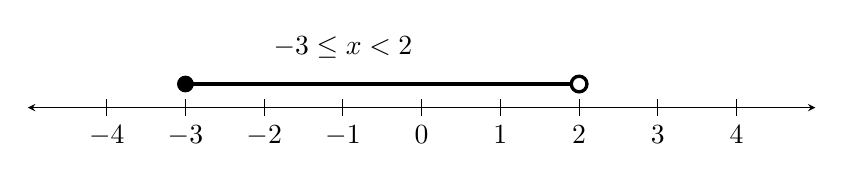
\begin{tikzpicture}

%drawing x-axis ticks
\foreach \x in  {-4,...,4}
\draw[shift={(\x,0)},color=black] (0pt,3pt) -- (0pt,-3pt);

%labeling x-axis ticks
\foreach \x in {-4,...,4}
\draw[shift={(\x,0)},color=black] (0pt,0pt) -- (0pt,-3pt) node[below] 
{$\x$};

%drawing the number line through ticks
\draw [very thin,black,stealth-stealth] (-5,0) -- (5,0); %stealth means a pointy arrow, so stealth-stealth has two

%draws a line segment with circle
\draw[very thick,black] (-3,0.3) -- (2,0.3)  node[fill=white,draw=black,circle, inner sep=2pt] at (2,0.3) {}; 

%draws just a circle
\draw node[fill=black,draw=black,circle, inner sep=2pt] at (-3,0.3) {};

%creates a label
\draw (-1,0.5) node[anchor=south] {$-3\le x<2$};

\end{tikzpicture}
    
\end{document}